\documentclass[11pt,letterpaper]{article}
\usepackage[margin=0.72in]{geometry}
\usepackage{amsmath,amssymb,graphicx,booktabs}
\usepackage[T1]{fontenc}
\usepackage{lmodern}
\usepackage[hidelinks]{hyperref}
\setlength{\parindent}{0pt}
\setlength{\parskip}{4pt}
\setlength{\abovedisplayskip}{6pt}
\setlength{\belowdisplayskip}{6pt}
\setlength{\abovedisplayshortskip}{4pt}
\setlength{\belowdisplayshortskip}{4pt}
\newcommand{\SourceCount}{100}
\newcommand{\Depth}{1}
\newcommand{\Ridge}{0.001}
\newcommand{\TeacherValidation}{8.63}
\newcommand{\DipoleValidation}{6.18}
\newcommand{\Improvement}{35.4}
\newcommand{\Correlations}{0.938,\ 0.908,\ 0.958}
\newcommand{\CutY}{-0.85}
\newcommand{\KernelLength}{0.35}
\newcommand{\KernelRidge}{0.1}
\newcommand{\TrainCount}{500}
\newcommand{\CandidateCount}{36}

\hypersetup{pdftitle={From a learned kernel to a magnetic field: real-data reconstruction with equivalent dipoles},
pdfauthor={J. R. Landers},
pdfsubject={A follow-up to From samples to an equation, using public magnetic measurements and a magnetostatic source representation}}
\begin{document}
\begin{center}
{\Large\bfseries From a learned kernel to a magnetic field}\\[3pt]
{\large Real-data reconstruction with equivalent dipoles}\\[3pt]
{\small J. R. Landers\quad$\cdot$\quad November 2026}
\end{center}
\vspace{-6pt}

\textbf{Starting question.}
Can a kernel learned from real magnetic measurements be converted into an explicit
magnetic-field function whose theoretical shapes predict unseen measurements?
The earlier note~[1] verified a workflow on a hidden synthetic field: samples
became a Gaussian kernel, then a differential equation, then its solved analytic
function. Here we test a different bridge: project a measured vector-field kernel
onto a family supplied by magnetostatic theory, and judge the result against
held-out measurements. There is no known analytic ground-truth curve for the room.

\textbf{1. Measurements become a vector-field kernel.}
The public Aalto recordings~[2] provide tracked planar positions and three
calibrated, orientation-corrected magnetic channels from a moving robot.
Let $\mathbf x_i=(x_i,y_i)$ be position in metres and $\mathbf b_i$ its measured
field vector. Each channel uses the same Gaussian similarity kernel:
\begin{equation}
\widehat{\mathbf B}_K(\mathbf x)=\overline{\mathbf B}
+\sum_i\boldsymbol\alpha_i k_\ell(\mathbf x,\mathbf x_i),\qquad
k_\ell(\mathbf x,\mathbf x_i)=
e^{-\|\mathbf x-\mathbf x_i\|^2/(2\ell^2)}.
\label{eq:kernel}
\end{equation}
The coefficient matrix is $(K+\rho I)^{-1}(Y-\mathbf1\overline{\mathbf B}^{\mathsf T})$,
where $Y$ stacks the measured vectors. Validation selects $\ell$ and $\rho$.
All field values retain the reference instrument's recording units; independent
SI calibration is unavailable. We use the full vector, retaining directional
information that a scalar magnitude profile discards.

\textbf{2. Theory supplies a magnetic response kernel.}
In static, source-free air with constant permeability, assume
$\nabla\cdot\mathbf B=0$ and $\nabla\times\mathbf B=0$.
Locally $\mathbf B=-\nabla\Phi$ with $\nabla^2\Phi=0$. An explicit harmonic potential is
\begin{equation}
\Phi(\mathbf r)=-\mathbf b_0\cdot\mathbf r+
\sum_{j=1}^{M}\frac{\mathbf q_j\cdot\mathbf R_j}{R_j^3},
\qquad \mathbf R_j=\mathbf r-\mathbf s_j,\quad R_j=\|\mathbf R_j\|.
\label{eq:potential}
\end{equation}
Here $\mathbf s_j$ is an equivalent source position, $\mathbf q_j$ its effective
dipole moment, and $\mathbf b_0$ a uniform background. Differentiating gives~[3]
\begin{equation}
\boxed{\ \mathbf B_D(\mathbf r)=\mathbf b_0+
\sum_{j=1}^{M}\underbrace{\left(
\frac{3\mathbf R_j\mathbf R_j^{\mathsf T}}{R_j^5}
-\frac{I_3}{R_j^3}\right)}_{\displaystyle D(\mathbf r,\mathbf s_j)}\mathbf q_j.\ }
\label{eq:dipoles}
\end{equation}
With SI calibration, $\mathbf q_j=\mu_0\mathbf m_j/(4\pi)$ for magnetic moment
$\mathbf m_j$; here this scale is absorbed into the fitted coefficients.
Every term satisfies the two assumed field equations away from its source.
The Gaussian $k_\ell$ measures similarity; the tensor $D$ maps source moments to
magnetic response. They are different kernels connected by the fit below.

For one vertical dipole at $(a,0,-h)$, evaluated on $(x,0,0)$,
\begin{equation}
B_z(x)=b_z+q\frac{2h^2-(x-a)^2}{[(x-a)^2+h^2]^{5/2}},\qquad
B_x(x)=b_x+3qh\frac{x-a}{[(x-a)^2+h^2]^{5/2}}.
\label{eq:shapes}
\end{equation}
Superposition produces peaks, troughs and sign changes without requiring one
monotone $\tanh$ curve. These shapes are supplied physics; their weights are inferred.

\newpage
\textbf{3. The learned kernel determines equivalent moments.}
Set the observation plane to $z=0$ and place a regular source grid at $z=-h$.
This is an assumed representation, not a measured floor depth. At the $n$ training
positions, stack the kernel predictions into $\mathbf t\in\mathbb R^{3n}$ and the
response blocks into $D\in\mathbb R^{3n\times3M}$.
Let $C$ subtract the per-component mean across positions, and let diagonal $S$
contain the column norms of $CD$. The implemented regularized projection is
\begin{align}
A&=CDS^{-1},\qquad
\widehat{\mathbf w}=
\underset{\mathbf w}{\arg\min}\bigl\{\|A\mathbf w-C\mathbf t\|_2^2
+\lambda\|\mathbf w\|_2^2\bigr\},\nonumber\\
\widehat{\mathbf q}&=S^{-1}(A^{\mathsf T}A+\lambda I)^{-1}A^{\mathsf T}C\mathbf t,
\qquad
\widehat{\mathbf b}_0=\operatorname{mean}_i
\left[\widehat{\mathbf B}_K(\mathbf x_i)-(D\widehat{\mathbf q})_i\right].
\label{eq:projection}
\end{align}
An SVD evaluates this expression. Substitution into Eq.~\eqref{eq:dipoles} produces
an explicit three-dimensional magnetic field, observed and tested on its planar
restriction. For fixed geometry and penalties this is a linear transformation
of the learned kernel's outputs. The background is unpenalized; column scaling
specifies the regularization convention. No measured currents or derivatives
are available, and no synthetic physical observations enter fitting.

\textbf{4. Real-data experiment.}
Use Invensense trials 1--2 for fitting, trial 3 for selection, trials 4--5 for
stable-environment evaluation, and trials 6--9 for changed-environment stress.
Training uses \TrainCount\ positions, capped at 250 per trial. Exclude
$[1.5,2.5]\times[-2,-1]$~m and a 0.15~m buffer from training and validation.
The original kernel selects $\ell=\KernelLength$~m and $\rho=\KernelRidge$.
Other instruments use the existing trial-1-only affine alignment to the reference
frame and scale. Evaluation uses the same measured observations for all models.

Fit moments only to kernel predictions at actual training positions. These targets
are derived model outputs, not additional observations. Search grid sides
$4,7,10$, depths $0.25,0.5,1$~m, and penalties $10^{-5},10^{-3},0.1,1$.
Choose minimum measured source-validation vector RMSE among the \CandidateCount\ candidates;
freeze all choices before scoring the test labels. Selection gives
\SourceCount\ dipoles at depth \Depth~m with $\lambda=\Ridge$: 303 fitted
coefficients including the background. Validation error falls from
\TeacherValidation\ to \DipoleValidation.

\textbf{5. Predictive results.}
Report vector error $\sqrt{N^{-1}\sum_i\|\mathbf b_i-\widehat{\mathbf B}_i\|_2^2}$,
in reference recording units. Stable trials 4--5 are pooled by instrument:
\begin{center}
\small\begin{tabular}{@{}lrrrr@{}}
\toprule
Instrument & Constant & Kernel & Kernel $\to$ dipoles & Direct dipoles \\
\midrule
Invensense & 16.48 & 8.09 & 5.22 & 5.31 \\
Nexus phone & 16.32 & 10.34 & 8.83 & 8.85 \\
Trivisio & 16.42 & 8.03 & 5.56 & 5.71 \\
\bottomrule
\end{tabular}

\end{center}
\vspace{-4pt}
The reconstructed field reduces source-instrument error by \Improvement\%.
Its three component correlations with measured test values are
$\Correlations$. A matched control fits moments directly to training
measurements at the same selected geometry and penalty. Its similar error shows
that the supplied physical representation accounts for much of the gain; the
kernel stage has not been shown necessary. The control is not separately optimized.

With the fitted fields frozen, changed-environment trials 6--9 give:
\begin{center}
\small\begin{tabular}{@{}lrrrr@{}}
\toprule
Instrument & Constant & Kernel & Kernel $\to$ dipoles & Direct dipoles \\
\midrule
Invensense & 17.62 & 8.64 & 7.33 & 7.36 \\
Nexus phone & 27.53 & 24.16 & 23.81 & 23.79 \\
Trivisio & 17.24 & 8.69 & 7.43 & 7.50 \\
\bottomrule
\end{tabular}

\end{center}
\vspace{-4pt}
The large phone errors remain visible. Neither predictor establishes transfer
across arbitrary environmental changes. These acquisitions were examined in earlier
experiments: this is exploratory test reuse, not a fresh confirmatory study.

\newpage
\textbf{6. Do the shapes agree?}
\begin{center}
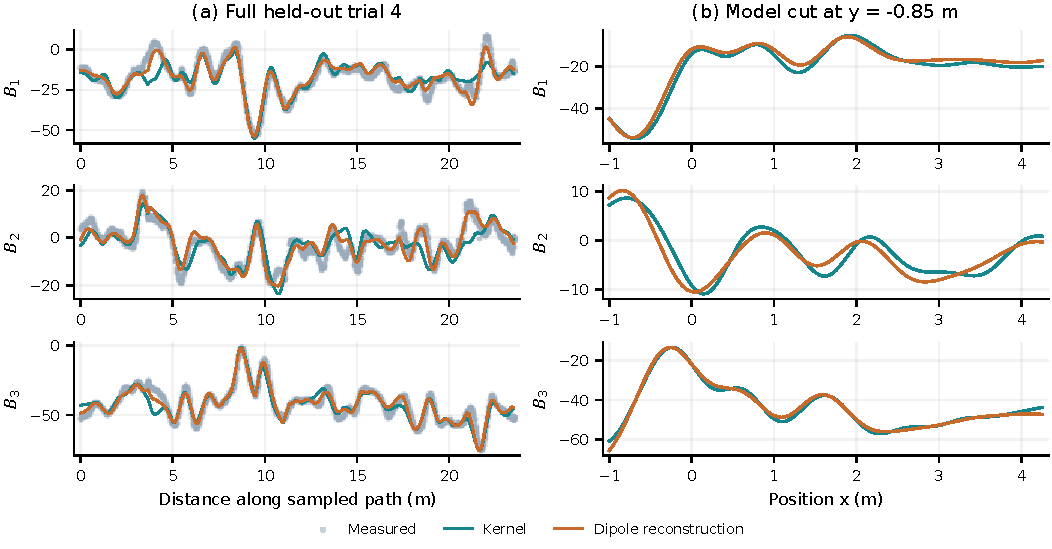
\includegraphics[width=\linewidth]{field_reconstruction.pdf}
\end{center}
\vspace{-9pt}
{\small\textbf{Figure 1.} All three field components, in reference recording units.
(a) The full first held-out acquisition, Invensense trial 4: measured values,
learned Gaussian kernel and equivalent dipole reconstruction. Distance is accumulated
between retained path positions. (b) A fixed model cut at $y=\CutY$~m, the median
training coordinate. The two reconstructed shapes agree broadly; no independent
measured ground-truth curve is available exactly on this cut. Tables pool both
stable test trials rather than selecting the displayed acquisition.}

\vspace{5pt}
\textbf{7. What has been derived?}
Equations~\eqref{eq:potential}--\eqref{eq:projection} give a complete route from
the real-data kernel to a theoretical magnetic-field function. The reconstructed
field obeys the supplied source-free magnetostatic equations away from the
equivalent sources, and predicts held-out values better than the original kernel
in this experiment. Three-dimensional curl and divergence identities were checked
numerically; saved coefficients reproduce the reported predictions and errors.

This differs from the earlier synthetic recovery~[1]. There, a restricted
equation search recovered the hidden function family and was scored against an
analytic oracle. Here, the physical family is supplied and its coefficients are
inferred. The evidence is agreement with measured values; satisfying the imposed
field equations does not independently discover them.

Planar measurements do not determine a unique three-dimensional continuation or
the actual source arrangement. The fitted dipoles are equivalent sources, not
identified room objects. Depth and grid size both reach the largest searched values,
so neither is an established physical estimate or an established search optimum.
Source-depth sensitivity, stability across training trials and independent public
data with three-dimensional positions are the next tests of robustness.

\vfill
{\footnotesize\raggedright
\textbf{References and reproducibility.}\par
[1] J.~R. Landers, \emph{From samples to an equation: A magnetic-like kernel benchmark}
(2026). \href{../01-kernel-to-equation/kernel_to_equation.pdf}{Companion note in \texttt{papers/01-kernel-to-equation/}}.\par
[2] A. Solin et al., \emph{Modeling and interpolation of the ambient magnetic field
by Gaussian processes}, IEEE Trans. Robotics (2018),
\href{https://doi.org/10.1109/TRO.2018.2830326}{doi:10.1109/TRO.2018.2830326}.
\href{https://github.com/AaltoML/magnetic-data}{Public recordings}; pinned archive,
upstream calibration and orientation correction retained.\par
[3] NASA CCMC, \href{https://ccmc.gsfc.nasa.gov/static/files/Dipole.pdf}{\emph{Potential Form of the Dipole Field Equations}}.\par
Build all notes: \texttt{python scripts/build\_papers.py}.
Protocol, coefficients, provenance and scores:
\texttt{experiments/magnetic\_mapping/dipole\_field/}.\par}
\end{document}
